\chapter{Some Infrastructure: Linear Algebra} 
\label{chap:linalg}  

There are some issues that will come up frequently.  We'll first cover them
briefly here, more later as the need arises.  This chapter will review
linear algebra, while the following one will review/extend the reader's
knowledge of probability and statistics.

RS methods, as with other machine learning (ML) techniques, often make
use of linear algebra, well beyond mere matrix multiplication. 

\section{Matrix Rank and Vector Linear Independence}

Consider the matrix

\begin{equation}
\label{rankex1}
M = 
\left (
\begin{array}{rrrr}
1 & 5 & 1 & -2 \\
8 & 3 & 2 & 8 \\
9 & 8 & 3 & 6 
\end{array}
\right )
\end{equation}

Note that the third row is the sum of the first two.  In many contexts,
this would imply that there are really only two ``independent'' rows in
$M$ in some sense related to the application.  

Denote the rows of $M$ by $r_i, ~ i = 1,2,3$.  Recall that we say they
are \textit{linearly independent} if it is not possible to find scalars
$a_i$, at least one of them nonzero, such that the \textit{linear
combination} $a_1 r_1 + a_2 r_2 + a_3 r_3$ is equal to 0.  In this case
$a_1 = a_2 = 1$ and $a_3 = -1$ gives us 0, so the rows of $M$ are
linearly dependent.

Recall that the \textit{rank} of a matrix is its maximal number of
linearly independent rows and columns.  (It can be shown that the row
rank and column rank are the same.)  The rank of $M$ above is 2.

Recall too the notion of the \textit{basis} of a vector space
$\mathcal{V}$.  It is a linearly independent set of vectors whose linear
combinations collectively form all of $\mathcal{V}$.  Here  $r_1$ and
$r_2$ form a basis for the \textit{row space} of $M$.  Alternatively,
$r_1$ and $r_3$ also form a basis, as do $r_2$ and $r_3$.

The rank of an $r \times s$ matrix is thus at most $\min(r,s)$.  In
the case of equality, we say the matrix has \textit{full rank}.  A
ratings matrix, such as $A$ in Section \ref{mf}, should be of full rank,
since there presumably are no exact dependencies among users or items.

\section{Partitioned Matrices}
\label{partmat}

It is often helpful to partition a matrix into \textit{blocks} (often
called {\it tiles} in the parallel computation community).

\subsection{How It Works}

Consider matrices $A$, $B$ and $C$,

\begin{equation}
A = 
\left (
\begin{array}{ccc}
1 & 5 & 12 \\
0 & 3 & 6 \\
4 & 8 & 2
\end{array}
\right )
\end{equation}

and

\begin{equation}
B = 
\left (
\begin{array}{ccc}
0 & 2 & 5 \\
0 & 9 & 10 \\
1 & 1 & 2
\end{array}
\right ), 
\end{equation}

so that

\begin{equation}
C = AB = 
\left (
\begin{array}{ccc}
12 & 59 & 79 \\
6 & 33 & 42 \\
2 & 82 & 104
\end{array}
\right ) .
\end{equation}

We could partition A as, say,

\begin{equation}
A =
\left (
\begin{array}{cc}
A_{11} & A_{12} \\
A_{21} & A_{22}
\end{array}
\right ) ,
\end{equation}

where

\begin{equation}
A_{11} =
\left (
\begin{array}{cc}
1 & 5 \\
0 & 3
\end{array}
\right )  ,
\end{equation}

\begin{equation}
A_{12} =
\left (
\begin{array}{cc}
12 \\
6 
\end{array}
\right ),
\end{equation}

\begin{equation}
A_{21} =
\left (
\begin{array}{cc}
4 & 8 
\end{array}
\right )  
\end{equation}

and

\begin{equation}
A_{22} =
\left (
\begin{array}{c}
2
\end{array}
\right ).
\end{equation}

Similarly we would partition B and C into blocks of a compatible size to A,

\begin{equation}
B =
\left (
\begin{array}{cc}
B_{11} & B_{12} \\
B_{21} & B_{22}
\end{array}
\right )
\end{equation}

\begin{equation}
C =
\left (
\begin{array}{cc}
C_{11} & C_{12} \\
C_{21} & C_{22}
\end{array}
\right ) ,
\end{equation}

so that for example

\begin{equation}
B_{21} =
\left (
\begin{array}{cc}
1 & 1
\end{array}
\right ) .
\end{equation}

The key point is that multiplication still works if we pretend that
those submatrices are numbers!  For example, pretending like that would
give the relation

\begin{equation}
C_{11} = A_{11} B_{11} + A_{12} B_{21}, 
\end{equation}

which the reader should verify really is correct as matrices, i.e. the
computation on the right side really does yield a matrix equal to $C_{11}$.

\subsection{Important Special Case}

Recall the relation 

\begin{equation}
\label{awh}
A \approx WH
\end{equation}

in Section \ref{mf}, where $A$ is $r \times s$, $W$ is $r \times m$ and
$H$ is $m \times s$.  Partition the first and third  matrices into rows, i.e.\
write


\begin{equation}
A =
\left (
\begin{array}{c}
a_1 \\
... \\
a_r 
\end{array}
\right ),
\end{equation}

and

\begin{equation}
H =
\left (
\begin{array}{c}
h_1 \\
... \\
h_m 
\end{array}
\right ),
\end{equation}

Keep $W$ unpartitiond:

\begin{equation}
W = 
\left (
\begin{array}{ccc}
w_{11} & ... & w_{1m}\\
... & ... & ... \\
w_{r1} & ... & w_{rm}
\end{array}
\right ),
\end{equation}

Using the partitioning idea, write $WH$ as a ``matrix-vector product'':

\begin{equation}
WH =
\left (
\begin{array}{ccc}
w_{11} & ... & w_{1m}\\
... & ... & ... \\
w_{r1} & ... & w_{rm}
\end{array}
\right )
\left (
\begin{array}{cc}
h_1 \\
... \\
h_m 
\end{array}
\right )
=
\left (
\begin{array}{cc}
w_{11}h_1 + ... + w_{1m} h_m \\
... \\
w_{r1}h_1 + ... + w_{rm} h_m \\
\end{array}
\right )
\end{equation}

Look at that!  What it says is row $i$ of $WH$, and thus approximately
row $i$ of $A$, is a linear combination of the rows of $H$.  And with a
different partitioning, we'd find that each column of $WH$ is a linear
combination of the columns of $H$.  We'll see in Chapter \ref{chap:svd}
that this has big implications for the matrix factorization method of
RS, a topic we lay the groundwork for next.

\section{The Notion of Approximate Rank:  Principal Components
Analysis}

Suppose the matrix in (\ref{rankex1}) had been

\begin{equation}
\label{rankex2}
M =
\left (
\begin{array}{rrrr}
1 & 5 & 1 & -2\\
8.02 & 2.99 & 2 & 8.2\\
9 & 8 & 3 & 6 
\end{array}
\right )
\end{equation}

Intuitively, we still might say that the rank of $M$ is
``approximately'' 2.  Or better yet, row 3 still seems redundant, Let's
formalize that, leading to one of the most common techniques in
statistics/machine learning.  By the way, this technique will also later
provide a way to find $W$ and $H$ in (\ref{awh}).

(Warning:  This section will be somewhat long, but quite central to
RS/ML.)

\subsection{Dimension Reduction}

One of the major themes in computer science is \textit{scale}, as in the
common question, ``Does it scale?''  The concern is, does an algorithm,
method or whatever work well in large-scale systems?

In the RS context, just think of, say, Amazon.  The business has
millions of users and millions of items.  In other words, the ratings
matrix has millions of rows and millions of columns, and even one
million rows and columns would mean a total number of $(10^6)^2 =
10^{12}$ entries, about 8 terabytes of data.

This is a core point in statistics/machine learning, the notion of
\textit{dimension reduction}.  In complex applications, there is a
pressing need to reduce the number of variables down to a 
manageable number --- manageable not only in terms of computational time
and space, but also the statistical problem of \textit{overfitting}
(Chapter \ref{chap:infra2}).

So we need methods to eliminate redundant or near-redundant data, such
as row 3 in (\ref{rankex2}).

\subsection{Exploiting Correlations}
\label{explorecorr}

Statistically, the issue is one of correlation.  In (\ref{rankex2}), the
third row is highly correlated with (the sum of) the first two rows.  To
explore the correlation idea further, here are two graphs of bivariate
normal densities:

\begin{minipage}[b]{0.65\linewidth}
    \mbox{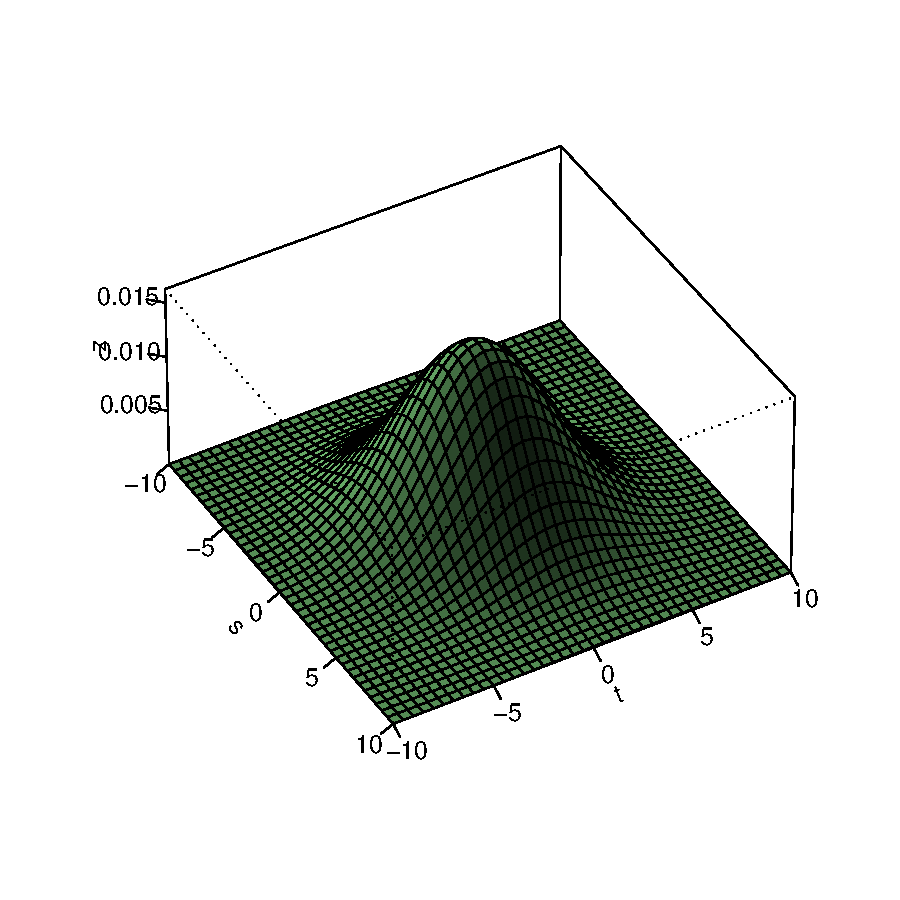
\includegraphics[width=3.25in]{Images/Rho2.pdf}} 
\end{minipage}
\hspace{0.0in}
\begin{minipage}[b]{0.65\linewidth}
    \mbox{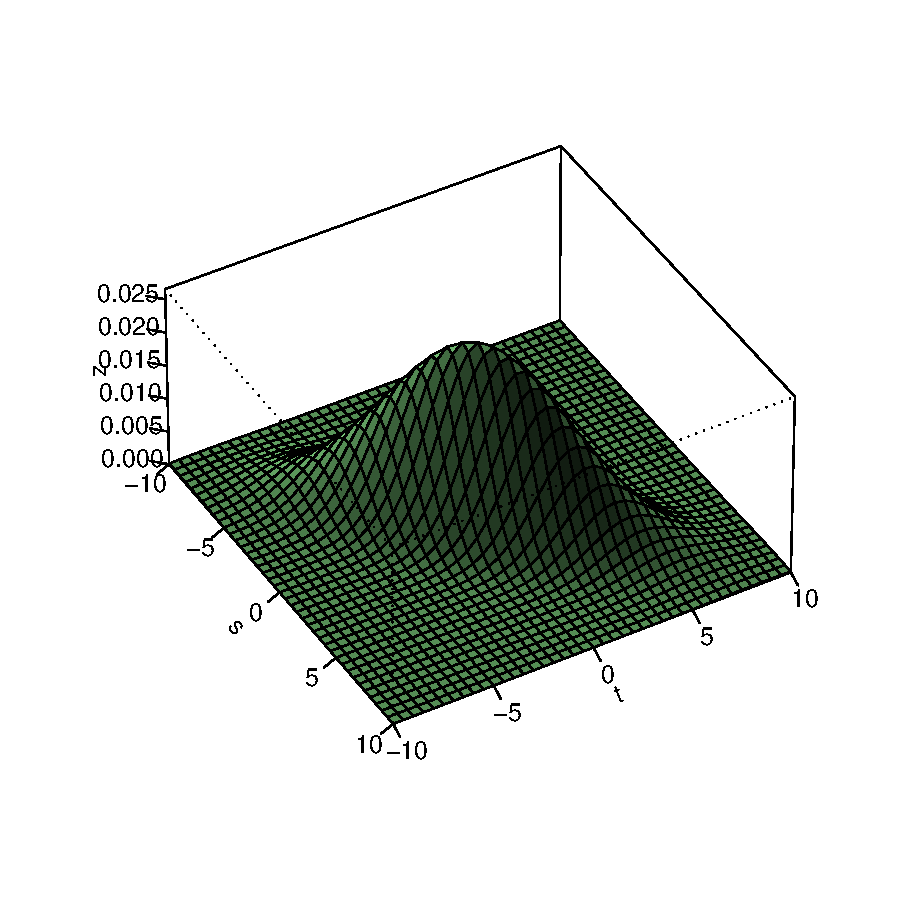
\includegraphics[width=3.25in]{Images/Rho8.pdf}} 
\end{minipage}

Let's call the two variables $X_1$ and $X_2$, with the corresponding
axes in the graphs to be referred to as $t_1$ and $t_2$.  The first
graph was generated with a correlation of 0.2 between the two variables,
while in the second one, the correlation is 0.8.

Not surprisingly due to the high correlation in the second graph, the
``two-dimensional bell'' is concentrated around a straight line,
specifically the line $t_2 = - t_1$.  In other words, there is high
probability that $X_2 \approx -X_1$, so that:  

\begin{quote}

To a large extent, there is only one variable here, $X_1$ (or other
choices, e.g.\ $X_2$), not two.  

\end{quote}

Note one more time, though, the approximate nature of the approach we
are developing.  There really \textit{are} two variables above.  By
using only one of them, \textbf{we are relinquishing some information.  But with
the need to avoid overfitting, use of the approximation may be a net win
for us.}

Well then, how can we determine a set of near-redundant variables, so
that we can consider omitting them from our analysis?  Let's look at
those graphs a little more closely.

Any \textit{level set} in the above graphs, i.e.\ a curve one
obtains by slicing the bells parallel to the $(t_1,t_2)$ plane can be
shown to be an ellipse.  As noted, the major axis of the ellipse will be
the line $t_1 + t_2 = 0$.  The minor axis will be the line perpendicular
to that, $t_1 - t_2 = 0$.  In turn, that means that standard probability
methods can then be used to show that the variables

\begin{equation}
Y_1 = X_1 + X_2 
\end{equation}

and 

\begin{equation}
Y_2 = X_1 - X_2 
\end{equation}

have 0 correlation.  Then we have a good case for using only $Y_1$ in
our data analysis, instead of using $X_1$ and $X_2$.  

But why not use just $X_1$?  As usual in statistics/ML, things get more
complicated in higher dimensions.  In choosing variables to retain in
our analysis, it makes sense to require that they be uncorrelated, as
$Y_1$ and $Y_2$ are above; if not, intuitively there is some redundancy
among them, which of course is what we are hoping to avoid.  

With that in mind, now suppose we have $p$ variables, $X_1,
X_2,...,X_p$, not just two.  We can no longer visualize in higher
dimensions, but one can show that the level sets will be 
$p$-dimensional ellipsoids.  These now have $p$ axes rather than just
two, and we can define $p$ new variables, $Y_1,Y_2,...,Y_p$ from the
$X_i$, such that:

\begin{itemize}

\item [(a)] The $Y_i$ are uncorrelated.

\item [(b)] We can order them in terms of variance:

\begin{equation}
Var(Y_1) > Var(Y_2) > ... > Var(Y_p)
\end{equation}

\end{itemize} 

Now we have a promising solution to our dimension reduction problem.
In [(b)] above, we can choose to use just the first few of the $Y_i$,
omitting the ones with small variance.  And again, since the $Y_i$ will
be uncorrelated, we are eliminating a source of possible redundancy
among them.

PCA won't be a perfect solution --- there is no such thing --- as might
be the case if the relations between variables is nonmonotonic.  A
common example is age, with mean income given age tending to be a
quadratic (or higher degree) polynomial relation.  But PCA is a very
common ``go to'' method for dimension reduction, and may work well even
in (mildly) nonmonotonic settings.

Now, how do we find these $Y_i$?

\subsection{Eigenanalysis}

Say I have a sample of $n$ observations on two variables, $x =
(x_1,...,x_n)$ and $y=(y_1,...,y_n$, say height and weight on $n = 100$
people.  Then, formally, the \textit{correlation} between the variables
is

\begin{equation}
\label{corrdef}
\frac
{\frac{1}{n} \sum_{i=1}^n (x_i-\overline{x}) (y_i-\overline{y})}
{s.d.(x) ~ s.d.(y)}
\end{equation}

where the denominator is the product of the sample standard deviations of the
two variables, and $\overline{x})$ and $\overline{y})$ are the sample
means.  The correlation is a number between -1 and 1.

The correlation matrix $C$ of a set of $p$ variables is $p \times p$, i.e.\
square.  Moreover, since $\textrm{corr}(X_i,X_j) = \textrm{corr}(X_j,X_i)$,
$C$ is \textit{symmetric}:

\begin{equation}
C' = C
\end{equation}

where $'$ denotes matrix transpose.  

Recall that for any square matrix $L$, if there is a scalar $\lambda$
and a nonzero vector $x$ such that 

\begin{equation}
Lx = \lambda x
\end{equation}

then we say that $x$ is an \textit{eigenvector} of $L$, with
\textit{eigenvalue} $\lambda$.  (Note that the above implies that $x$ is
a column vector, $p \times 1$, a convention we will use throughout the
book.)

It can be shown that any symmetric matrix has real (not complex)
eigenvalues, and that the corresponding eigenvectors $U_1,...,U_p$
are orthogonal,

\begin{equation}
U_i' U_j = 0, ~ i \neq j
\end{equation}

We always take the $U_i$ to have length 1.

\subsection{PCA}

Typically we have many cases in our data, say $n$, arranged in an $n
\times p$ matrix $Q$, with row $i$ representing case $i$ and column $j$
representing the $j^{th}$ variable.

Say our data is about people, 1000 of them, and we have data on height,
weight, age, gender, years of schooling and income.  Then $n = 1000$, $p
= 6$.

So, finally, here is PCA:

\begin{enumerate}


\item Find the correlation matrix (or covariance matrix, a similar notion)
from the data in $Q$.  Note that since there are $p$, the correlation
matrix will be $p \times p$.

\item Compute its eigenvalues and eigenvectors.  

\item After ordering the eigenvalues from largest to smallest, let
$\lambda_i$ be the $i^{th}$ largest, and let $U_i$ be the corresponding
eigenvector, scaled to have length 1.  

\item Let $U$ be the matrix whose $i^{th}$ column is $U_i$.  Its size
will be $p \times s$.

\item Choose the first few eigenvalues, say $s$ of them, using some
criterion (see below).  Denote the matrix of the first $s$ columns of $U$
by $U^{(s)}$.  Note that $U$ is 

\item Form a new data matrix, 

\begin{equation}
\label{rqu}
R = Q U^{(s)}
\end{equation}

$R$ will be of size $n \times s$.  Column $j$ of $R$ is called the
$j^{th}$ principal component of the original data.  

It will be shown below that the variance of the $j^{th}$ principal
component is $\lambda_j$.  The sum of all $p$ values is the same as the
sum of the variances of the original variables, an important point.

\end{enumerate} 

From this point onward, any data analysis we do will be with $R$, not
$Q$.  In $R$, row $i$ is still data on the $i^{th}$ case, e.g. the
$i^{th}$ person, but now with $s$ new variables in place of the original
$p$.  Since typically $s << p$, we have achieved considerable dimension
reduction.

\subsection{Matrix View}

Using the approach of Section \ref{partmat}, write

\begin{equation}
R = Q U^{(s)} = Q (U_1,...,U_s) = (QU_1,...,QU_s)
\end{equation}

where as before the $U_i$ are the eigenvectors

So, the $i^{th}$ column of $R$ is $Q U_i$.  The latter quantity, again
by Section \ref{partmat}, is a linear combination of the columns of $Q$,
with the coefficients in that linear combination being the elements in
$U_i$.  Recall that each column of $Q$ is one variable; e.g.\ for
people, there may be an age column, a height column, a weight column and
so on.  Each column in $R$ is one of our new variables.  Therefore:

\begin{quote}
The $i^{th}$ new variable is equal to a linear combination of the old
variables.
\end{quote}

So, a new variable might be, say, 1.9 age + 0.3 height + 1.2 weight.

\subsection{Why It Works}

Recall that the new variables have the $\lambda_i$ for variances and are
uncorrelated.  Here's why:

It is common to \textit{center} and \textbf{scale} one's data, meaning
to subtract from each variable its mean, and divide by its standard
deviation.  The new mean and standard deviation are 0 and 1.  In that
case, (\ref{corrdef}) becomes


\begin{equation}
\frac{1}{n} \sum_{i=1}^n x_i y_i
\end{equation}

The reader should verify that with the matrices $Q$ and $R$ above (old
and new data), their correlation matrices are $Q'Q$ and $R'R$.  Let's
see how that works out:

\begin{eqnarray}
\label{rrqq}
R'R &=& (Q U^{(s)})' (QU^{(s)}) \\  
&=&  
U^{(s)} {}' Q' ~ Q U^{(s)} \\
\end{eqnarray}

using the fact that $(AB)' = B'A'$.

But remember that the $U_i$ are eigenvectors of the correlation matrix,
in this case $Q'Q$!  So

\begin{equation}
\label{qqu}
Q'Q U^{(s)} = (\lambda_1 U_1,...,\lambda_s U_s)
\end{equation}

Finally, recall that the $U_i$ are orthogonal with length 1.
Substituting (\ref{qqu}) in $rrqq$, we then get

\begin{equation}
R'R = \textrm{diag}(\lambda_1,...,\lambda_s)
\end{equation}

the matrix having the $\lambda_i$ on the diagonal and 0s elsewhere.  The
latter imply that the new variables are uncorrelated, and the former
fact says that the variances of the new variables are the $\lambda_i$,
as claimed.

\subsection{Choosing the Number of Principal Components}

So, how do we choose $s$?  This is the hard part, and there is no 
universal good method.  Typically $s$ is chosen so that 

\begin{equation}
\sum_{j=1}^s \lambda_j
\end{equation}

is ``most'' of total variance (again, that total is the above expression
with $p$ instead of $s$), but even this is usually done informally.

In ML/RS settings, though, $s$ is typically chosen by a technique called
\textit{cross validation}, to be discussed in Chapter \ref{chap:infra2}.

\subsection{Software and Example}

The most commonly used R function for PCA is \textbf{prcomp()}.  As with
many R functions, it has many optional arguments; we'll take the default
values here.

For our example, let's use the Turkish Teaching Evaluation data,
available from the UC Irvine Machine Learning Data Repository.  It
consists of 5820 student evaluations of university instructors.  Each
student evaluation consists of answers to 28 questions, each calling for
a rating of 1-5, plus some other variables we won't consider here.

\begin{lstlisting}
> turk <- read.csv('turkiye-student-evaluation.csv',header=T)
> head(turk)
  instr class nb.repeat attendance difficulty Q1 Q2 Q3 Q4
1     1     2         1          0          4  3  3  3  3
2     1     2         1          1          3  3  3  3  3
3     1     2         1          2          4  5  5  5  5
4     1     2         1          1          3  3  3  3  3
5     1     2         1          0          1  1  1  1  1
6     1     2         1          3          3  4  4  4  4
  Q5 Q6 Q7 Q8 Q9 Q10 Q11 Q12 Q13 Q14 Q15 Q16 Q17 Q18 Q19
1  3  3  3  3  3   3   3   3   3   3   3   3   3   3   3
2  3  3  3  3  3   3   3   3   3   3   3   3   3   3   3
3  5  5  5  5  5   5   5   5   5   5   5   5   5   5   5
4  3  3  3  3  3   3   3   3   3   3   3   3   3   3   3
5  1  1  1  1  1   1   1   1   1   1   1   1   1   1   1
6  4  4  4  4  4   4   4   4   4   4   4   4   4   4   4
  Q20 Q21 Q22 Q23 Q24 Q25 Q26 Q27 Q28
1   3   3   3   3   3   3   3   3   3
2   3   3   3   3   3   3   3   3   3
3   5   5   5   5   5   5   5   5   5
4   3   3   3   3   3   3   3   3   3
5   1   1   1   1   1   1   1   1   1
6   4   4   4   4   4   4   4   4   4
> tpca <- prcomp(turk[,-(1:5)]
\end{lstlisting}

Let's explore the output.  First, the standard deviations of the new
variables:

\begin{lstlisting}
> tpca$sdev
 [1] 6.1294752 1.4366581 0.8169210 0.7663429 0.6881709
 [6] 0.6528149 0.5776757 0.5460676 0.5270327 0.4827412
[11] 0.4776421 0.4714887 0.4449105 0.4364215 0.4327540
[16] 0.4236855 0.4182859 0.4053242 0.3937768 0.3895587
[21] 0.3707312 0.3674430 0.3618074 0.3527829 0.3379096
[26] 0.3312691 0.2979928 0.2888057
> tmp <- cumsum(tpca$sdev^2)
> tmp / tmp[28]
 [1] 0.8219815 0.8671382 0.8817389 0.8945877 0.9049489
 [6] 0.9142727 0.9215737 0.9280977 0.9341747 0.9392732
[11] 0.9442646 0.9491282 0.9534589 0.9576259 0.9617232
[16] 0.9656506 0.9694785 0.9730729 0.9764653 0.9797855
[21] 0.9827925 0.9857464 0.9886104 0.9913333 0.9938314
[26] 0.9962324 0.9981752 1.0000000
\end{lstlisting}

This is striking,  The first principal component (PC) already accounts
for 82\% of the total variance among all 28 questions.  The first five
PCs cover over 90\%.  This suggests that the designer of the evaluation
survey could have written a much more concise survey instrument with
almost the same utility.

Now keep in mind that each PC here is essentially a ``super-question''
capturing student opinion via a weighted sum of the original 28
questions.  Let's look at the first two PCs' weights:

\begin{lstlisting}
> tpca$rotation[,1]
        Q1         Q2         Q3         Q4         Q5 
-0.1787291 -0.1869604 -0.1821853 -0.1841701 -0.1902141 
        Q6         Q7         Q8         Q9        Q10 
-0.1870812 -0.1878324 -0.1867865 -0.1823915 -0.1923626 
       Q11        Q12        Q13        Q14        Q15 
-0.1866948 -0.1862382 -0.1922729 -0.1911814 -0.1902380 
       Q16        Q17        Q18        Q19        Q20 
-0.1962885 -0.1808833 -0.1935788 -0.1927359 -0.1931985 
       Q21        Q22        Q23        Q24        Q25 
-0.1911060 -0.1908591 -0.1948393 -0.1931334 -0.1888957 
       Q26        Q27        Q28 
-0.1908694 -0.1897555 -0.1886699 
\end{lstlisting}

\begin{lstlisting}

> tpca$rotation[,2]
         Q1          Q2          Q3          Q4          Q5 
 0.35645673  0.23223504  0.11551155  0.24533527  0.20717759 
         Q6          Q7          Q8          Q9         Q10 
 0.20075314  0.24290761  0.24901577  0.12919618  0.18911720 
        Q11         Q12         Q13         Q14         Q15 
 0.11051480  0.21203229 -0.10616030 -0.15629705 -0.15533847 
        Q16         Q17         Q18         Q19         Q20 
-0.04865706 -0.26259518 -0.12905840 -0.15363392 -0.19670071 
        Q21         Q22         Q23         Q24         Q25 
-0.22007368 -0.22347198 -0.10278122 -0.06210583 -0.20787213 
        Q26         Q27         Q28 
-0.12045026 -0.07204024 -0.21401477 
\end{lstlisting}

The first PC turned out to place approximately equal weights on all 28
questions.  The second PC, though, placed its heaviest weight on Q1,
with substantially varying weights on the other questions.

While we are here, let's check that the columns of $U$ are orthogonal.

\begin{lstlisting}
> t(tpca$rotation[,1]) %*% tpca$rotation[,2]
              [,1]
[1,] -2.012279e-16
\end{lstlisting}

Yes, 0 (with roundoff error).  As an exercise in matrix partitioning,
the reader should run

\begin{lstlisting}
t(tpca$rotation) %*% tpca$rotation
\end{lstlisting}

then check that it produces the identity matrix $I$, then ponder why
this should be the case.
